

%-------------------------------------------------------------------------------
% Dokumenten Klasse
\documentclass[
	final,
	a4paper,
	oneside,
	parskip=full,
	headings=standardclasses,
	headings=big,
	pointlessnumbers
]{scrartcl}

%-------------------------------------------------------------------------------
% Packete nutzen
\usepackage{ngerman,palatino,setspace}
\usepackage[T1]{fontenc}
\usepackage[latin9]{inputenc}
\usepackage[left=25mm,right=25mm,top=25mm,bottom=25mm]{geometry}
\usepackage{graphicx}
\usepackage{scrpage2}
\usepackage{listings}
\usepackage[usenames,dvipsnames,svgnames]{xcolor}
\usepackage[hidelinks]{hyperref}
\usepackage{caption}
\usepackage{mdframed}
\usepackage{dashbox}
\usepackage{cancel}
\usepackage{csquotes}

\usepackage{multirow}% http://ctan.org/pkg/multirow
\usepackage{hhline}% http://ctan.org/pkg/hhline


%\renewcommand{\thesection}{\arabic{section}}
%\renewcommand{\thesubsection}{\arabic{section}.\arabic{subsection}}
%\renewcommand{\thesubsubsection}{\arabic{section}.\arabic{subsection}.\arabic{subsubsection}} 
%\renewcommand{\thesubsection}{\Roman{section}.\alph{subsection})}
\renewcommand{\thesection}{\arabic{section}.}
\renewcommand{\thesubsection}{\arabic{section}.\alph{subsection})}

%-------------------------------------------------------------------------------
% Hintergrundfarbe von Packet 'framed' mit Kommando 'shaded' nutzen
\colorlet{shadecolor}{gray!25}

%-------------------------------------------------------------------------------
% F�r "align" Umgebung eine Zelle nach links/rechzs verschieben
\makeatletter
\newcommand{\pushright}[1]{\ifmeasuring@#1\else\omit\hfill$\displaystyle#1$\fi\ignorespaces}
\newcommand{\pushleft}[1]{\ifmeasuring@#1\else\omit$\displaystyle#1$\hfill\fi\ignorespaces}
\makeatother

%-------------------------------------------------------------------------------
% Mathematik
\usepackage{amsmath}
\usepackage{amssymb}
\usepackage{mathtools}

%-------------------------------------------------------------------------------
% Kopf- und Fusszeile

\pagestyle{scrheadings}
\clearscrheadfoot
\cfoot[Seite \thepage]{Seite \thepage}

%-------------------------------------------------------------------------------
% Bilder
\newenvironment{Figure}
{\par\medskip\noindent\minipage{\linewidth}}
{\endminipage\par\medskip}

%%% EINHEITEN %%%%%%%%%%%%%%%%%%%%%%%5%%%%%%%%%%%%%%%%%%%%%%%%%%%%%%%%%%%%%%%%%%
\usepackage[
separate-uncertainty  = true,
output-decimal-marker ={.},
repeatunits           = false,
range-phrase          = {\,bis\,},
]{siunitx}

%-------------------------------------------------------------------------------
%
\date{\today}

%-------------------------------------------------------------------------------
% Dokumenten Einstellungen

% Section Abst�nde
\RedeclareSectionCommand[
	beforeskip=-1\baselineskip,
	afterskip=0.001\baselineskip
]{section}
\RedeclareSectionCommand[
	beforeskip=0\baselineskip,
	afterskip=0.001\baselineskip
]{subsection}

% Formeln
\DeclareCaptionType{mycapequ}[aa][bb]
\captionsetup[mycapequ]{labelformat=empty}

\def\changemargin#1#2{\list{}{\rightmargin#2\leftmargin#1}\item[]}
\let\endchangemargin=\endlist 

%-------------------------------------------------------------------------------
% Listings
\lstset{
	language=Matlab,
	breaklines=true,
	numbers=left,
	numberstyle=\tiny,
	numbersep=5pt,
	captionpos=b,
	basicstyle=\footnotesize\ttfamily,
	stringstyle=\color{magenta},
	identifierstyle=\color{black},
	keywordstyle=\color{blue}, 
	commentstyle=\color{DarkGreen}
}

\newcommand{\mylisting}[2][]{%
	\lstinputlisting[caption={\texttt{\detokenize{#2}}},#1]{#2}%
}

%-------------------------------------------------------------------------------
% Dokument
\begin{document}
	
	\section{Blutsenkung}
	Erythrozyten als Kugelvolumen
	
	\begin{mycapequ}[!ht]
		\vspace{-0.5cm}
		\begin{align*}
			%% 0
			\text{Kugelradius}              && r            &= \; ? \\
			%% 1
			\text{Kugelvolumen}             && V_{K}        &= \frac{4}{3} \pi r^3 \\
			%% 2
			\text{Gewichtskraft}            && F_G          &= V_K \cdot \rho_K \cdot g \\
			%% 3
			\text{Auftriebskraft}           && F_A          &= V_K \cdot \rho_i \cdot g \\
			%% 4
			\text{Viskose Reibung}          && F_R          &= 6 \pi \cdot r \cdot \eta \cdot v \\
			%% 5
			\text{Gleichgewicht}            && F            &= F_A + F_R - F_G = m \cdot a = 0 \\
			%% 6
			\text{Viskosit�t}               && \eta         &= 1.73 \cdot 10^{-3} \mathrm{\;Pa\;s} \\
			%% 7
			\text{Dichte Erythozyten}       && \rho_{K}     &= 1.096 \; \frac{\mathrm{g}}{\mathrm{cm}^3} 
			= 1096 \; \frac{\mathrm{kg}}{\mathrm{m}^3} \\
			%% 8
			\text{Dichte Plasma}            && \rho_{i}     &= 1.027 \; \frac{\mathrm{g}}{\mathrm{cm}^3}
			= 1027 \; \frac{\mathrm{kg}}{\mathrm{m}^3} \\
			%% 9
			\text{Senkungsgeschwindigkeit}  && v            &= 10 \; \frac{\mathrm{mm}}{\mathrm{h}}
			= 2.777 \cdot 10^{-6} \; \frac{\mathrm{m}}{\mathrm{s}} \\
			%% 10
			\text{Fallbeschleunigung}       && g            &= 9.81 \; \frac{\mathrm{m}}{\mathrm{s}^2}
		\end{align*}
		\vspace{-0.5cm}
	\end{mycapequ}
	
	\begin{mycapequ}[!ht]
		\vspace{-0.5cm}
		\begin{align*}
			%% 1
			F = F_A + F_R - F_G &= 0 \\
			%% 2
			\left(V_K \cdot \rho_i \cdot g\right) +
			\left( 6 \pi \cdot r \cdot \eta \cdot v \right) -
			\left( V_K \cdot \rho_K \cdot g \right) &= 0 \\
			%% 3
			\left( \left[ \frac{4}{3} \pi r^3 \right] \cdot \rho_K \cdot g \right) -
			\left( \left[ \frac{4}{3} \pi r^3 \right] \cdot \rho_i \cdot g\right) &=
			\left( 6 \pi \cdot r \cdot \eta \cdot v \right) \\
			%% 4
			r^2 \cdot \left[ \left(  \frac{4}{3} \pi \cdot \rho_K \cdot g \right) -
			\left( \frac{4}{3} \pi \cdot \rho_i \cdot g\right) \right] &=
			6 \pi \cdot \eta \cdot v \\
			%% 5
			r &= \sqrt{\frac{6 \pi \cdot \eta \cdot v}{\frac{4}{3} \pi \cdot \rho_K \cdot g  -
					\frac{4}{3} \pi \cdot \rho_i \cdot g }} \\
			%% 6
			r &= \sqrt{\frac{6 \cancel{\pi} \cdot \eta \cdot v}
				{\frac{4}{3} \cancel{\pi} \cdot g \cdot \left(\rho_K - \rho_i \right)}} \\
			%% 7
			r &= \sqrt{\frac{9 \cdot \eta \cdot v}
				{2 \cdot g \cdot \left(\rho_K - \rho_i \right)}} \\
			%% 8
			r &= \sqrt{\frac{9 \cdot 1.73 \cdot 10^{-3} \frac{kg}{m \cdot s} \cdot 2.777 \cdot 10^{-6} \; \frac{\mathrm{m}}{\mathrm{s}}}
				{2 \cdot 9.81 \; \frac{\mathrm{m}}{\mathrm{s}^2} \cdot \left(1096 \; \frac{\mathrm{kg}}{\mathrm{m}^3} - 1027 \; \frac{\mathrm{kg}}{\mathrm{m}^3} \right)}} \\
			%% 9
			\left[ r^2 \right] &= \frac{\frac{\mathrm{kg}}{\mathrm{m} \cdot \mathrm{s}} \cdot \frac{\mathrm{m}}{\mathrm{s}}}
			{\frac{\mathrm{m}}{\mathrm{s}^2} \cdot \frac{\mathrm{kg}}{\mathrm{m}^3}} =
			\frac{\cancel{kg} \cdot \cancel{m}\cdot \cancel{s^2} \cdot m^3}{\cancel{m} \cdot \cancel{s^2} \cdot m \cdot \cancel{kg}} = \mathrm{m}^2\\
			%% 10
			r &= \sqrt{3.194 \cdot 10^{-11} \; \mathrm{m}^2} \\
			%% 11
			r &= 5.651 \cdot 10^{-6} \; \mathrm{m} = 5.651 \; \mu\mathrm{m} \\
			%% 12
			r_{\mathrm{Wikipedia}} &= 3.75 \; \mu\mathrm{m}
		\end{align*}
		\vspace{-0.5cm}
	\end{mycapequ}
	
	\newpage
	\section{Gleichgewichtsreaktion}
	
		\subsection{L�sen der Bindungsreaktions-Differentialgleichung}
	
			Die DGL ist wie folgt:
			\begin{mycapequ}[!ht]
				\vspace{-0.7cm}
				\begin{alignat}{3}
					\frac{d}{dt}\Gamma\left(t\right) &= \frac{d}{dt}\Gamma_\textrm{on}\left(t\right) && - \frac{d}{dt}\Gamma_\textrm{off}\left(t\right) \\
					\frac{d}{dt}\Gamma\left(t\right) &= k_\textrm{on} \cdot c \cdot \left( \Gamma_\textrm{max} - \Gamma\left(t\right)\right) && - k_\textrm{off} \cdot \Gamma\left(t\right)
				\end{alignat}
				\vspace{-0.7cm}
			\end{mycapequ}
		
			\begin{mycapequ}[!ht]
				\begin{mdframed}[leftmargin=0cm,
					skipabove=1cm,    
					linecolor=black,
					backgroundcolor=gray!10,
					linewidth=0.75pt,
					innerleftmargin=0em,
					innerrightmargin=0em,
					innertopmargin=0.75em,
					innerbottommargin=0.5em,
					]
					\begin{addmargin}[1em]{2em}% 1em left, 2em right
						\textbf{Integration einer Differentialgleichung durch Substitution}
						
						\vspace{-0.50cm}
						\begin{align*}
							y\mkern3mu' & = f\left(a x + b y + c \right) \\
						\end{align*}
						\vspace{-1.00cm}
						
						Mit Hilfe einer \textit{geeignete Substitution} kann sie auf eine
						\textit{separable} Differentialgleichung 1. Ordnung zur�ckgef�hrt werden.
						
						\vspace{-0.50cm}
						\begin{align*}
							u  & = a \; x + b \; y + c \\
							u\mkern3mu' & = a + b \; y\mkern3mu' \\
							u\mkern3mu' - a & = b \; y' \\
							\frac{u\mkern3mu' - a}{b} & = y' \\
							\frac{u\mkern3mu' - a}{b} & = f \left( u \right)
						\end{align*}
						%\vspace{-1.00cm}
						
					\end{addmargin}
				\end{mdframed}
			\end{mycapequ}
		
			L�sen durch Substitution
			\begin{mycapequ}[!ht]
				\vspace{-0.7cm}
				\begin{alignat}{5}
					%% 1.
					\Gamma\mkern3mu' &= k_\textrm{on} \cdot c \cdot \left( \Gamma_\textrm{max} - \Gamma\right) - k_\textrm{off} \cdot \Gamma \span \span \span \span \label{eq:1}  \\
					%% 2
					u                & = c && + && \; b \; y && + a \; x\\
					%% 3
					u                & = c && + && \; b \; \Gamma && + a \; t\\
					%% 4
					u                &= k_\textrm{on} \cdot c \cdot \Gamma_\textrm{max} \; && - && \; k_\textrm{on} \cdot c \cdot \Gamma - k_\textrm{off} \cdot \Gamma \label{eq:4}\\
					%% 5
					u &= k_\textrm{on} \cdot c \cdot \Gamma_\textrm{max} \; && - && \; \left( k_\textrm{on} \cdot c \cdot + k_\textrm{off} \right) \cdot \Gamma \label{eq:5} \\
					%% 6
					u\mkern3mu' &=  &&- && \; \left( k_\textrm{on} \cdot c \cdot + k_\textrm{off} \right) \cdot \Gamma\mkern3mu' \\
					%% 7
					\frac{- u\mkern3mu'}{k_\textrm{on} \cdot c \cdot + k_\textrm{off}} &=  &&  && \; \Gamma\mkern3mu' \label{eq:7} 
				\end{alignat}
				\vspace{-0.7cm}
			\end{mycapequ}
		
			Gleichsetzen von \eqref{eq:7} mit \eqref{eq:1} respektive \eqref{eq:4}, Trennen der Variablen und Integrieren
			
			\begin{mycapequ}[!ht]
				\vspace{-0.7cm}
				\begin{alignat}{5}
					%% 1
					u &= \frac{- \dbox{$u\mkern3mu'$}}{k_\textrm{on} \cdot c \cdot + k_\textrm{off}} \\
					%% 2
					- \left(k_\textrm{on} \cdot c \cdot + k_\textrm{off} \right) \cdot u &= \dbox{$\frac{1}{dt} \cdot du$} \\
					%% 3
					- \left(k_\textrm{on} \cdot c \cdot + k_\textrm{off} \right) \cdot \int{1 \cdot dt} &= \int{\frac{1}{u} \cdot du} \\
					%% 4
					- \left(k_\textrm{on} \cdot c \cdot + k_\textrm{off} \right) \cdot t + C_1 &= \ln \left(u\right) \\
					%% 5
					C_2 \cdot e^{- \left(k_\textrm{on} \cdot c \cdot + k_\textrm{off} \right) \cdot t} &= u
				\end{alignat}
				\vspace{-0.7cm}
			\end{mycapequ}
		
			\newpage
			
			R�cksubstituieren von $u$ mit \eqref{eq:5}
			
			\begin{mycapequ}[!ht]
				\vspace{-0.5cm}
				\begin{alignat}{5}
					%% 1
					C_2 \cdot e^{- \left(k_\textrm{on} \cdot c \cdot + k_\textrm{off} \right) \cdot t} &= u \\
					%% 2
					C_2 \cdot e^{- \left(k_\textrm{on} \cdot c \cdot + k_\textrm{off} \right) \cdot t} &= k_\textrm{on} \cdot c \cdot \Gamma_\textrm{max} \; && - && \; \left( k_\textrm{on} \cdot c \cdot + k_\textrm{off} \right) \cdot \Gamma \\
					%% 3
					\left( k_\textrm{on} \cdot c \cdot + k_\textrm{off} \right) \cdot \Gamma &= k_\textrm{on} \cdot c \cdot \Gamma_\textrm{max} \; && - && \; C_2 \cdot e^{- \left(k_\textrm{on} \cdot c \cdot + k_\textrm{off} \right) \cdot t} \\
					%% 4
					\Gamma \left(t\right)&= \frac{k_\textrm{on} \cdot c \cdot \Gamma_\textrm{max}}{k_\textrm{on} \cdot c + k_\textrm{off}} \; && - && \; \frac{C_2 \cdot e^{- \left(k_\textrm{on} \cdot c \cdot + k_\textrm{off} \right) \cdot t}}{k_\textrm{on} \cdot c + k_\textrm{off}} \\
				\end{alignat}
				\vspace{-0.5cm}
			\end{mycapequ}
		
			Konstante $C_2$ bestimmen durch Anfangswert $ \Gamma \left(0\right) = 0$
			
			\begin{mycapequ}[!ht]
				\vspace{-0.5cm}
				\begin{align*}
						%% 1
						\Gamma \left(0\right)&= 0 = \frac{k_\textrm{on} \cdot c \cdot \Gamma_\textrm{max}}{k_\textrm{on} \cdot c + k_\textrm{off}} - \frac{C_2 \cdot \overbrace{e^{0}}^{=1}}{k_\textrm{on} \cdot c + k_\textrm{off}} \\
						%% 1
						\frac{C_2}{k_\textrm{on} \cdot c + k_\textrm{off}} &= \frac{k_\textrm{on} \cdot c \cdot \Gamma_\textrm{max}}{k_\textrm{on} \cdot c + k_\textrm{off}} \\
						%% 2
						C_2 &= k_\textrm{on} \cdot c \cdot \Gamma_\textrm{max}
				\end{align*}
				\vspace{-0.5cm}
			\end{mycapequ}
			
			Die L�sung mit Anfangswert $ \Gamma \left(0\right) = 0$ lautet wie folgt
		
			\begin{mycapequ}[!ht]
				\vspace{-0.5cm}
				\begin{align*}
					%% 1
					\Gamma \left(t\right)&= \frac{k_\textrm{on} \cdot c \cdot \Gamma_\textrm{max}}{k_\textrm{on} \cdot c + k_\textrm{off}} - \frac{k_\textrm{on} \cdot c \cdot \Gamma_\textrm{max} \cdot e^{- \left(k_\textrm{on} \cdot c \cdot + k_\textrm{off} \right) \cdot t}}{k_\textrm{on} \cdot c + k_\textrm{off}} \\
					%% 2
					\Gamma \left(t\right)&= \frac{k_\textrm{on} \cdot c \cdot \Gamma_\textrm{max}}{k_\textrm{on} \cdot c + k_\textrm{off}} \cdot \left( 1 - e^{- \left(k_\textrm{on} \cdot c \cdot + k_\textrm{off} \right) \cdot t}\right) \\
					%% 3
					\Gamma \left(t\right)&= \Gamma_\textrm{max} \cdot \frac{c }{c + \frac{k_\textrm{off}}{k_\textrm{on}}} \cdot \left( 1 - e^{- \left(k_\textrm{on} \cdot c \cdot + k_\textrm{off} \right) \cdot t}\right) \\
				\end{align*}
				\vspace{-0.5cm}
			\end{mycapequ}
		
			Gleichgewicht bestimmen
			
			\begin{mycapequ}[!ht]
				\vspace{-0.5cm}
				\begin{align*}
					%% 1
					\frac{d}{dt}\Gamma\left(t\right) &= 0 \\
					%% 2
					 0 &= k_\textrm{on} \cdot c \cdot \left( \Gamma_\textrm{max} - \Gamma_{\textrm{Gleichgewicht}} \right) - k_\textrm{off} \cdot \Gamma_{\textrm{Gleichgewicht}} \\
					%% 3
					0 &= k_\textrm{on} \cdot c \cdot \Gamma_\textrm{max} - k_\textrm{on} \cdot c \cdot \Gamma_{\textrm{Gleichgewicht}} - k_\textrm{off} \cdot \Gamma_{\textrm{Gleichgewicht}} \\
					%% 4
					0 &= k_\textrm{on} \cdot c \cdot \Gamma_\textrm{max} - \left( k_\textrm{on} \cdot c \cdot + k_\textrm{off} \right) \cdot \Gamma_{\textrm{Gleichgewicht}} \\
					%% 5
					\left( k_\textrm{on} \cdot c \cdot + k_\textrm{off} \right) \cdot \Gamma_{\textrm{Gleichgewicht}} &= k_\textrm{on} \cdot c \cdot \Gamma_\textrm{max} \\
					%% 6
					\Gamma_{\textrm{Gleichgewicht}} &= \frac{k_\textrm{on} \cdot c \cdot \Gamma_\textrm{max}}{k_\textrm{on} \cdot c \cdot + k_\textrm{off}} \\
					%% 7
					\Gamma_{\textrm{Gleichgewicht}} &= \Gamma_\textrm{max} \cdot \frac{c }{c + \frac{k_\textrm{off}}{k_\textrm{on}}}
				\end{align*}
				\vspace{-0.5cm}
			\end{mycapequ}
	
	
		\newpage
		\subsection{Gleiches $K_D$, eine Gr�ssenordnung h�heres $k_{\mathrm{off}}$}
			\begin{labeling}{$k_{\mathrm{off}}$}
				\setlength{\itemsep}{0mm}
				\setlength{\parskip}{0.5mm}
				\setlength{\parindent}{0mm}
				\item[$k_{\mathrm{on}}$] Rate der freien Ligangen, die sich an Rezeptoren binden.
				\item[$k_{\mathrm{off}}$] Rate der gebundenen Ligangen, die sich von den Rezeptoren l�sen.
				\item[$K_D$] Verh�ltnis von $\frac{k_{\mathrm{off}}}{k_{\mathrm{on}}}$.
			\end{labeling}
			Da $K_D$ sich nicht �ndert, muss auch $k_{\mathrm{on}}$ eine Gr�ssenordnung h�her sein. \\
			Kleines $k_{\mathrm{on}}$ und $k_{\mathrm{off}}$: Langsame Rate f�r die Bindung und L�sung der Liganden. \\
			Grosses $k_{\mathrm{on}}$ und $k_{\mathrm{off}}$: Schnelle Rate f�r die Bindung und L�sung der Liganden. \\
		
		\subsection{Kleinste Konzentration $c$ bestimmen}
		Massenbelegung $\Gamma$ \\
		Maximale Massenbelegung $\Gamma_{\mathrm{max}}$\\
		Stoffmengenkonzentrationen (Liganden in L�sung) $c$
		
		\begin{mycapequ}[!ht]
			\vspace{-0.5cm}
			\begin{align*}
			%% 1
			c                                &= \;? \\
			%% 2
			K_D                              &= \frac{k_{\mathrm{off}}}{k_{\mathrm{on}}} = \frac{1}{10^{11}} = 1 \cdot 10^{-11} \; \frac{\mathrm{mol}}{\mathrm{m}^3} \\
			%% 3
			\shortintertext{Ansatz}
			\frac{d}{dt}\Gamma\left(t\right) &= |1| \; \frac{\mathrm{pg}}{\mathrm{mm}^2} = |0.001| \; \frac{\mathrm{ng}}{\mathrm{mm}^2}\\
			%% 4
			|0.001| \; \frac{\mathrm{ng}}{\mathrm{mm}^2} &= k_\textrm{on} \cdot c \cdot \left( \Gamma_\textrm{max} - \Gamma \right) - k_\textrm{off} \cdot \Gamma \tag*{$\Rightarrow$ \parbox{4.5cm}{Nicht Zielf�hrend, da $\Gamma$ nicht bekannt}}\\
			%% 5
			\shortintertext{Neuer Ansatz}
			\Gamma_{\textrm{Gleichgewicht}} \left( c \right) &= \Gamma_\textrm{max} \cdot \frac{c}{c + K_D} \\
			%% 6
			\frac{d}{dc} \Gamma \left( c \right) &= \Gamma_\textrm{max} \cdot \frac{K_D}{\left(c + K_D\right)^2} = | 0.001 | \; \frac{\mathrm{ng}}{\mathrm{mm}^2} \\
			%% 7
			\left(c + K_D\right)^2 &= \Gamma_\textrm{max} \cdot \frac{K_D}{| 0.001 | \; \frac{\mathrm{ng}}{\mathrm{mm}^2}} \\
			%% 8
			c &= \sqrt{\Gamma_\textrm{max} \cdot \frac{K_D}{| 0.001 | \; \frac{\mathrm{ng}}{\mathrm{mm}^2}}} - K_D
			\tag*{$\Rightarrow$ \parbox{4.5cm}{Nicht Zielf�hrend, da schon im Gleichgewicht}}\\
			\end{align*}
			\vspace{-0.5cm}
		\end{mycapequ}
	
		\begin{displayquote}
			Mit optischen Verfahren k�nnen �nderungen in der Massenbelegung ($\frac{d}{dt}\Gamma\left(t\right)$ ?) von $1 \; \frac{\mathrm{pg}}{\mathrm{mm}^2}$
			noch eindeutig nachgewiesen werden. Was ist die kleinste Konzentration (Stoffmengenkonzentrationen $c$) von Antigenen,
			welche man mit dieser Anordnung noch detektieren kann?
		\end{displayquote}
		�nderungen in der Massenbelegung ist nicht konstant. Wie kann ich da eine Konzentration berechnen?
		Jede Kurve flacht ab und die �nderungen der Massenbelegung geht gegen Null.
		
		\begin{Figure}
			\centering
			\includegraphics[width=14cm]{massenbelegung_kon.eps}
			\captionof{figure}{Ver�nderung von $k_{\mathrm{on}}$}
		\end{Figure}
	
		
		\begin{Figure}
			\centering
			\includegraphics[width=14cm]{massenbelegung_c.eps}
			\captionof{figure}{Ver�nderung von $c$}
		\end{Figure}
	
	\newpage
	\section{Sensitivit�t / Spezifit�t}
		
		\subsection{Mit Worten}
		\textbf{``Goldstandard''}\\
		\textit{diagnostische Spezifit�t}: Gesund diagnostizierte bei einer Gruppe von gesunden Probanden. \\
		\textit{diagnostische Sensitivit�t}: Krank diagnostizierte bei einer Gruppe von kranken Probanden.
		
		\subsection{Berechnen}
		\begin{centering}
			\includegraphics[trim={0.5cm 25cm 9cm 0.5cm},clip,width=14cm]{tuberkulosetest.pdf}
			\captionof{figure}{Wahrscheinlichkeitsbaum}
		\end{centering}
		
		Berechne WSK, dass negatives Testergebnis auch bedeutet, dass keine Erkrankung vorliegt.
		\begin{mycapequ}[!ht]
			\vspace{-0.5cm}
			\begin{align*}
				%% 1
				P\left(A\right) &= \frac{\mathrm{tn}}{\text{alle negativen}} = \frac{\mathrm{tn}}{\mathrm{tn} + \mathrm{fn}}
				                 = \frac{0.8 \cdot 0.99}{0.8 \cdot 0.99 + 0.2 \cdot 0.7} \\
				P\left(A\right) &= 0.848 \approx 85\%
			\end{align*}
			\vspace{-0.5cm}
		\end{mycapequ}
		
	\newpage
	\section*{Formeln und Tafeln}
		
		\begin{center}
			\renewcommand{\arraystretch}{1.5}
			\begin{tabular}{ | l | l | l | p{3.75cm} | }
				\multicolumn{1}{l}{\bfseries Name} &
				\multicolumn{1}{l}{\bfseries FZ} &
				\multicolumn{1}{l}{\bfseries Einheit}  &
				\multicolumn{1}{l}{\bfseries Formel } \\ \hline
				Kraft                      & $F$         & $N$, $\frac{kg \cdot m}{s^2}$  & $F = m \cdot a $ \\ \hline
				Druck                      & $p$         & $Pa$, $\frac{N}{m^2}$  & $p = \frac{F}{A}$ \\ \hline
				Dichte                     & $\rho$      & $\frac{kg}{m^3}$         & $\rho=\frac{m}{V}$ \\ \hline
				Viskosit�t                 & $\eta$      & $Pa \cdot s$, $\frac{kg}{m \cdot s}$ & \\ \hline
				Molek�lmasse               & $m_M$       & $kg$, $g$                & \\ \hline
				Avogadro-Konstante         & $N_A$       & $\frac{1}{mol}$          & \\ \hline
				Teilchenanzahl             & $N$         & -                        & 
				$ N = n \cdot N_A$ \\ \hline
				Stoffmenge                 & $n$         & $mol$                   
				& $n_{\mathrm{H}_2\mathrm{O}} = 
				\frac{m_{\mathrm{H}_2\mathrm{O}}}{M_{\mathrm{H}_2\mathrm{O}}} = \newline
				\frac{\SI{9}{g}}{\SI{18}{\frac{g}{mol}}} =
				\SI{0.5}{mol}$\\ \hline
				Molare Masse               & $m$         & $\frac{kg}{mol}$, $\frac{g}{mol}$ 
				& $M = \frac{m}{n} = N_A \cdot m_M$ \newline 
				$M_{\mathrm{H}_2\mathrm{O}} = 18.01528 \frac{g}{mol}$\\ \hline
				Stoffmengenkonzentrationen & $c$         & $\frac{mol}{m^3}$       
				& $c_i = \frac{n_i}{V} $ \\ \hline
				Massenbelegung             & $\Gamma$    & $\frac{kg}{m^2}$,  $\frac{g}{mm^2}$
				& $\Gamma = \frac{m}{A} $\\ \hline
				Str�mungsgeschwindigkeit   & $v$         & $\frac{m}{s}$                      
				& \\ \hline
				Gesetz von Stokes          & $F_R$       & $N$                      
				& $F_R = 6 \pi \cdot r \cdot \eta \cdot v $ \\ \hline
			\end{tabular}
			\captionof{table}{Formeln}
			\label{tab:materials}
		\end{center}
		
		
		\begin{Figure}
			\centering
			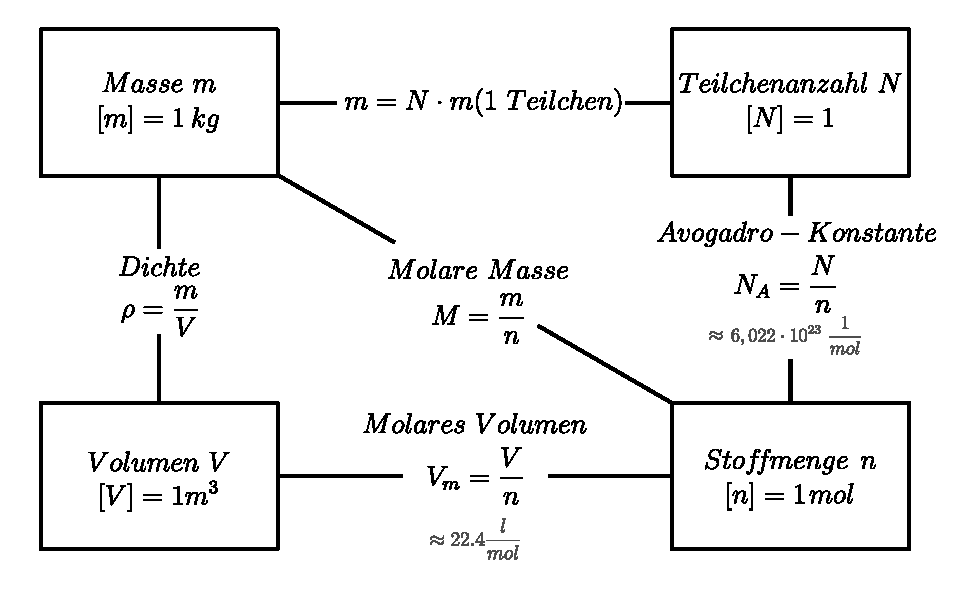
\includegraphics[width=15cm]{Stoffmenge.pdf}
			\captionof{figure}{Stoffmengen Umrechnung}
			\label{fig:drawing_compare}
		\end{Figure}
\end{document}
